\section{Siamese Multi-Object Tracking and Re-identification}
\label{sec:SiamMOTandReID}

% ##############################################################################
\subsection{Motivation}

% ##############################################################################
\subsection{Preliminary Discussion}

To make a full disclosure right at the beginning, we expected that the adoption of \gls{reid} enhancements within the \siammot{} framework would bring improvements in certain areas. Retrospectively, our experiments showed detrimental effects upon the tracker accuracy. In this section, we will elaborate further on why it is so in order to learn from such an experience as much as possible. Our surprise stems primarily from the fact that our thesis goals largely revolved around the application of \gls{reid} in object tracking. Therefore, finding that such approach does not yield the desired outcome raises multiple questions, namely the following ones:
\begin{enumerate}
    \item Does the inclusion of \gls{reid} into \gls{mot} frameworks have a potential to resolve cases of full occlusion without exacerbating other areas?
    \item Is the \gls{reid} extension suitable to the chosen \gls{mot} model, specifically, the \siammot{} tracker?
    \item Is the target use case in terms of datasets adequate to showcase the potential of \gls{reid} applied in the \siammot{} tracker?
\end{enumerate}
In our dicussion, we will answer these questions. Despite our negative outcome, we still consider the performed research to be a contribution to the \gls{mot} area.

% ##############################################################################
\subsection{Proposed ReID-Enhanced Architecture}
\label{ssec:ProposedReIDEnhancedArchitecture}

We adopted the object \gls{reid} architecture published in~\cite{luo2019bagoftricksreid} by Luo~\etal{}. The authors proposed a simple yet very robust framework for person \gls{reid}. We adopted this architecture (see \figtext{}~\ref{fig:BagOfTricksReIDArchitecture}) for vehicle \gls{reid} due to its simplicity accompanied with \gls{sota} performance at the time of publishing.

% ------------------------------------------------------------------------------
\begin{figure}[!t]
    \centering
    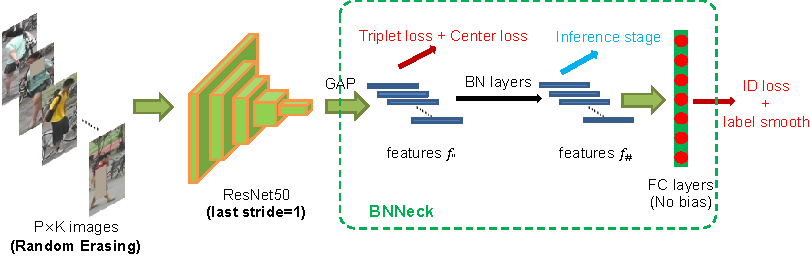
\includegraphics[width=\linewidth]{figures/methodology/bagoftricks_reid_architecture.pdf}
    \caption[Gls{reid} baseline]{A object \gls{reid} baseline which we used for our experiments. \externalsrc{\cite{luo2019bagoftricksreid}}}
    \label{fig:BagOfTricksReIDArchitecture}
\end{figure}
% ------------------------------------------------------------------------------

% ##############################################################################
\subsection{Training Phase}

% ##############################################################################
\subsection{Inference Phase}

The online solver algorithm was, from our point of view, the primary suspect for potential improvements due to its inherent simplicity that we considered inferior compared to the rest of the architecture.

% ##############################################################################
\subsection{Experimental Evaluation}

% ##############################################################################
\subsection{Discussion}